\documentclass[10pt,twocolumn,hidelinks,letterpaper]{article}

\usepackage[table]{xcolor}
\usepackage{cvpr}
\usepackage{times}
\usepackage{epsfig}
\usepackage{graphicx}
\usepackage{amsmath}
\usepackage{amssymb}

\usepackage[utf8x]{inputenc}
\usepackage[english]{babel}
\usepackage{url}
\usepackage{lipsum}

\usepackage[framed , numbered]{matlab-prettifier}
\usepackage{listings}
\usepackage{setspace}
\usepackage{color} %red, green, blue, yellow, cyan, magenta, black, white
\usepackage{geometry}
\usepackage{subcaption}
\usepackage{graphicx}
\usepackage{float}


% Include other packages here, before hyperref.

% If you comment hyperref and then uncomment it, you should delete
% egpaper.aux before re-running latex.  (Or just hit 'q' on the first latex
% run, let it finish, and you should be clear).
\usepackage[breaklinks=true,bookmarks=false]{hyperref}

\cvprfinalcopy % *** Uncomment this line for the final submission

\def\cvprPaperID{****} % *** Enter the CVPR Paper ID here
\def\httilde{\mbox{\tt\raisebox{-.5ex}{\symbol{126}}}}

% Pages are numbered in submission mode, and unnumbered in camera-ready
%\ifcvprfinal\pagestyle{empty}\fi
\setcounter{page}{1}
\begin{document}

%%%%%%%%% TITLE
\title{01TXFSM - Machine Learning and Deep Learning \\
\vspace{0.3in}
Final Project \\
First Person Action Recognition}

\author{
  Eros Fanì - s269781\\
  Politecnico di Torino\\
  {\tt\small eros.fani@studenti.polito.it}
  \and
  Gabriele Trivigno - s276807\\
  Politecnico di Torino\\
  {\tt\small gabriele.trivigno@studenti.polito.it}
  \and
  Cristiano Gerbino - s277058\\
  Politecnico di Torino\\
  {\tt\small s277058@studenti.polito.it}
}

\maketitle
%\thispagestyle{empty}

\lstset{language=python,%
  %basicstyle=\color{red},
  breaklines=true,%
  morekeywords={matlab2tikz},
  keywordstyle={\small \color{blue}},%
  morekeywords=[2]{1}, keywordstyle=[2]{\small \color{black}},
  identifierstyle={\small \color{black}},%
  stringstyle={\small \color{mylilas}},
  commentstyle={\small \color{mygreen}},%
  showstringspaces=false,%without this there will be a symbol in the places where there is a space
  numbers=left,%
  numberstyle={\small \color{black}},% size of the numbers
  numbersep=7pt, % this defines how far the numbers are from the text
  emph=[1]{error,warning},emphstyle=[1]{\small \color{red}} %some words to emphasise
  %emph=[2]{word1,word2}, emphstyle=[2]{style},
}

%%%%%%%%% BODY TEXT
\newcommand{\quotes}[1]{“#1”}
\newcommand{\reff}[1]{Figure \ref{#1}}
\setlength{\parindent}{0pt}
\setstretch{0.1}
\setlength{\parskip}{1em}
\definecolor{TopRow}{HTML}{E6E6FF}

\begin{abstract}


\end{abstract}

\section{Introduction}

\subsection{Goals}

The first goal of the project is to replicate some of the experiments performed in \cite{egornn} and \cite{sparnet}. The objective of these studies is the First Person Action Recognition: they tried to implement a deep learning model capable to extract meaningful features to automatically predict the action filmed by a wearable camera.

After having replicated these experiments we performed a grid search on the experiments to find the best set of values for the hyperparameters.

At last we have tried to improve the performances of the results of \cite{egornn} and \cite{sparnet} with some innovative ideas.

\subsection{Data exploration}

The dataset under analysis is a modified version of GTEA61\footnote{Georgia Tech Egocentric Activity Datasets: \small{\url{http://cbs.ic.gatech.edu/fpv/}}}. The dataset contains the videos in form of frames, and also two kind of preprocessed images: \textit{motion maps} and \textit{optical flows}. The folder schema of the dataset is shown in \reff{folder_schema}. Videos represent 61 class actions performed by 4 different users (\textit{S1}, \textit{S2}, \textit{S3}, \textit{S4}). Sometimes for some actions more than one video is available. The total number of videos in the dataset is, however, 457, which actually means that it is a quite small dataset.

\begin{figure*}
	\centering
	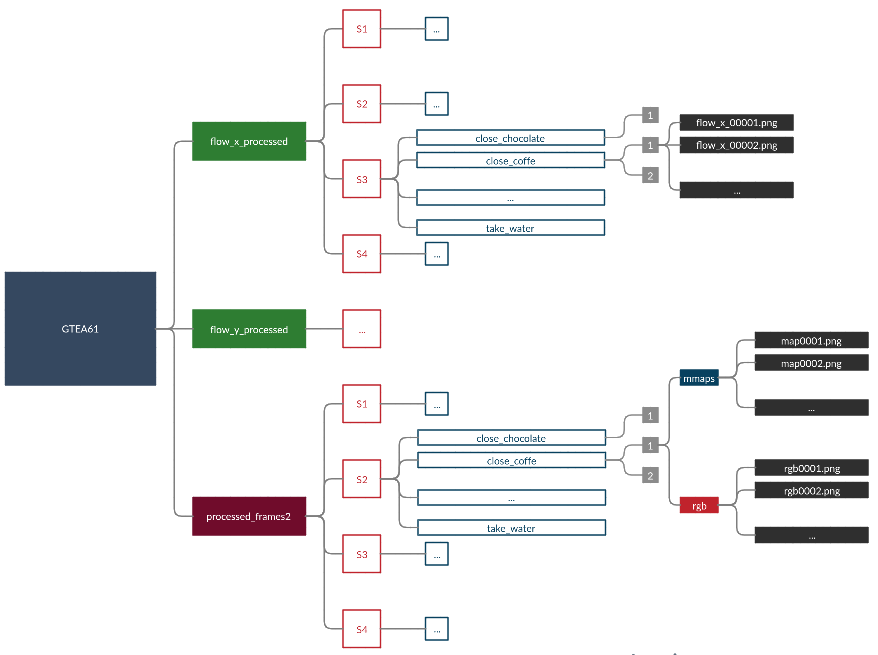
\includegraphics[width=.9\linewidth]{images/folder_schema.png}
	\caption{Folder schema of our GTEA61}
	\label{folder_schema}
\end{figure*}

The optical flow methods try to calculate the motion between two image frames which are taken at times $t$ and $t + \Delta t$ at every voxel position. The warp flow methods try also to remove the motion of the wearable camera. We have two kind of these last representations in our dataset: one computed in the horizontal axis (folder \textit{flow\_x\_processed}) and one other computed in the vertical axis (folder \textit{flow\_y\_processed}).

The motion maps are special black-and-white images which represent the spatial location in which the Motion Segmentation task of \cite{sparnet} focuses its attention per each frame. The mmaps present large similarities with the warp flows.

The differences between the kind of available images in our dataset are shown in \reff{image_comparison}.

\begin{figure*}
  \centering
  \begin{subfigure}{.24\linewidth}
  	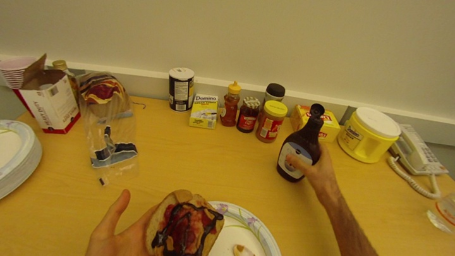
\includegraphics[width=\linewidth]{images/img_comp/rgb0001.png}
  \end{subfigure}
  \begin{subfigure}{.24\linewidth}
  	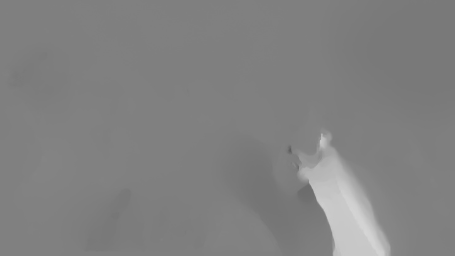
\includegraphics[width=\linewidth]{images/img_comp/flow_x_00002.png}
  \end{subfigure}
  \begin{subfigure}{.24\linewidth}
  	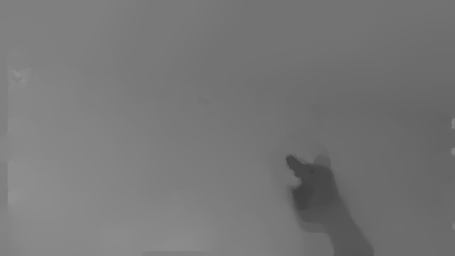
\includegraphics[width=\linewidth]{images/img_comp/flow_y_00001.png}
  \end{subfigure}
  \begin{subfigure}{.24\linewidth}
  	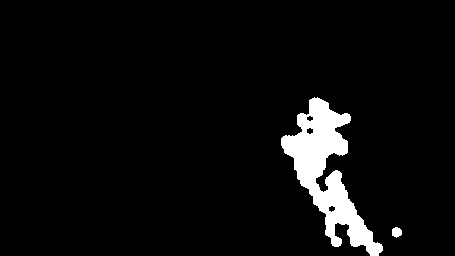
\includegraphics[width=\linewidth]{images/img_comp/map0001.png}
  \end{subfigure}
  \begin{subfigure}{.24\linewidth}
  	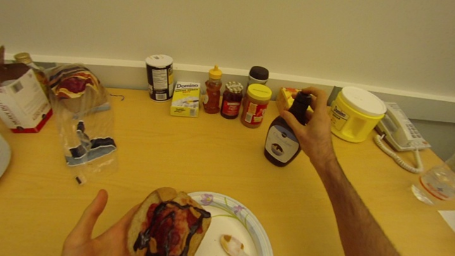
\includegraphics[width=\linewidth]{images/img_comp/rgb0011.png}
  \end{subfigure}
  \begin{subfigure}{.24\linewidth}
  	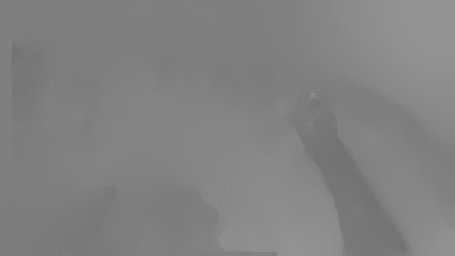
\includegraphics[width=\linewidth]{images/img_comp/flow_x_00011.png}
  \end{subfigure}
  \begin{subfigure}{.24\linewidth}
  	
\includegraphics[width=\linewidth]{images/img_comp/flow_y_00011.png}
  \end{subfigure}
  \begin{subfigure}{.24\linewidth}
  	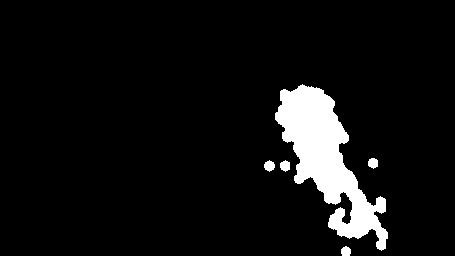
\includegraphics[width=\linewidth]{images/img_comp/map0011.png}
  \end{subfigure}
  \begin{subfigure}{.24\linewidth}
  	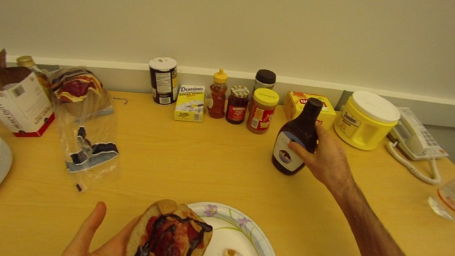
\includegraphics[width=\linewidth]{images/img_comp/rgb0020.png}
  \end{subfigure}
  \begin{subfigure}{.24\linewidth}
  	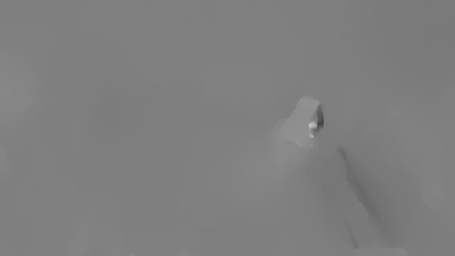
\includegraphics[width=\linewidth]{images/img_comp/flow_x_00020.png}
  \end{subfigure}
  \begin{subfigure}{.24\linewidth}
  	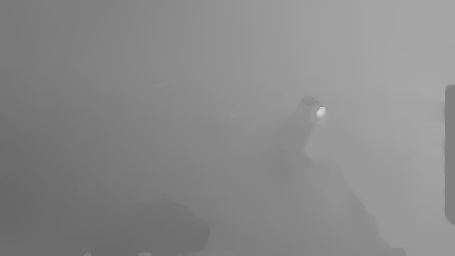
\includegraphics[width=\linewidth]{images/img_comp/flow_y_00020.png}
  \end{subfigure}
  \begin{subfigure}{.24\linewidth}
  	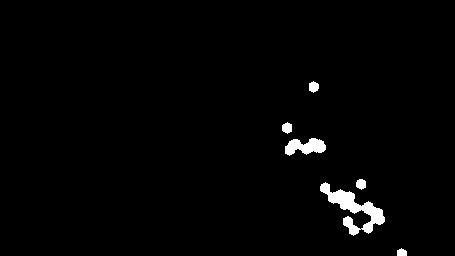
\includegraphics[width=\linewidth]{images/img_comp/map0020.png}
  \end{subfigure}
  \caption{Types of images in our dataset. In this example is shown a sample of images from the \textit{close\_chocolate} action. From the left column to the right column: rgbs, warp flows x, warp flows y, motion maps}
  \label{image_comparison}
\end{figure*}

\subsection{Data cleaning}

{\small
\bibliographystyle{ieee}
\bibliography{egbib}
}

\end{document}
